\documentclass[
    paper=a4,
    DIV14,
    fontsize=12pt,
    pagesize=pdftex,
    toc=bibliographynumbered
]{scrartcl}
\usepackage[utf8]{inputenc}
\usepackage[T1]{fontenc}
\usepackage[ngerman]{babel}
% \enquote{..} für automatische Anführungszeichen
\usepackage[autostyle=true]{csquotes}
% zusätzliche Optionen für Aufzählumgebungen itemize, enumerate, ..
\usepackage{enumitem}
% mathematische Symbole und Umgebungen
\usepackage{mathtools, amsfonts, amssymb, amsthm}

% Fonts
\usepackage{lmodern}
\usepackage{dsfont}

% Aussehen von Figuren
\usepackage[%
    font=footnotesize,
    margin=0.2em,
    labelfont=bf,
    format=plain,
    labelsep=endash
]{caption}
% Ermöglicht Anordnen von Unterfiguren
\usepackage[%
    font=footnotesize,
    margin=0.2em,
    labelfont=bf,
    format=plain,
    labelsep=endash
]{subcaption}

% Ermögliche Hyperlinks und anklickbare Referenzen
\usepackage{hyperref}

% stelle Fonts auf Serif
\setkomafont{sectioning}{\rmfamily\bfseries\boldmath}
\setkomafont{descriptionlabel}{\rmfamily\bfseries}
\numberwithin{figure}{section}
\numberwithin{equation}{section}
\numberwithin{table}{section}

% Mengen, wahrscheinlich nicht notwendig
\newcommand*\setZ{\mathds{Z}}
\newcommand*\setR{\mathds{R}}
\newcommand*\setN{\mathds{N}}
\newcommand*\setK{\mathds{K}}

% nummeriere besimmte Gleichungen
\newcommand\numberthis{\addtocounter{equation}{1}\tag{\theequation}}

% Matrizen, Vektoren
\newcommand*\vecz[2]{\begin{pmatrix} #1 \\ #2 \end{pmatrix}}
\newcommand*\vecd[3]{\begin{pmatrix} #1 \\ #2 \\ #3 \end{pmatrix}}
\newcommand*\vecf[4]{\begin{pmatrix} #1 \\ #2 \\ #3 \\ #4 \end{pmatrix}}
\newcommand*\matDD[4]{\begin{pmatrix} #1 & #2 \\ #3 & #4 \end{pmatrix}}

% Titel etc.
\title{Immer der Sonn' entgegen}
\subtitle{Proseminar: Mathematische Modellierung}
\author{Dominik Bendle \and Melissa Hasel \and Thomas Hofmann}
\date{Wintersemester 2016/17}

\begin{document}
\begin{titlepage}
    \maketitle
    \thispagestyle{empty}
    \centering
    \vfill
    % hier passendes Bild einfügen
    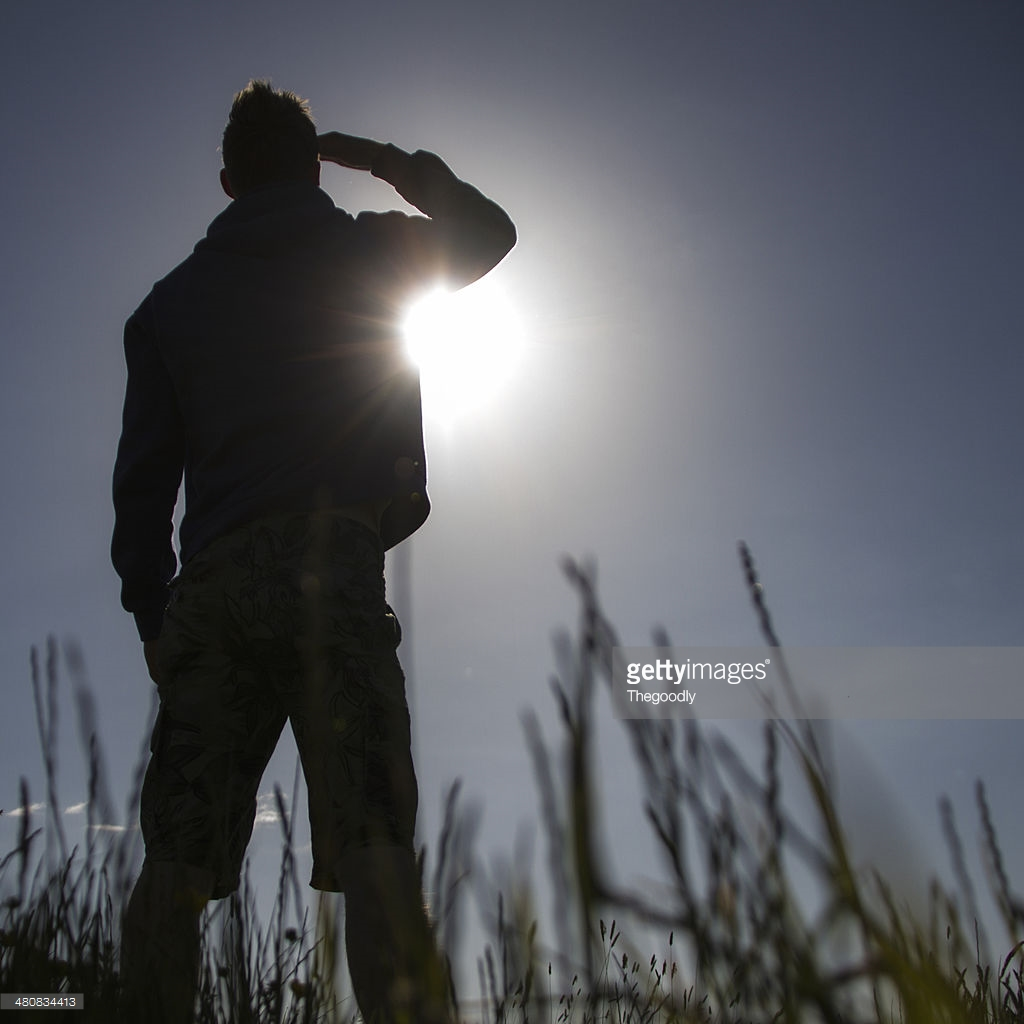
\includegraphics[width=0.7\textwidth]{images/man_looking_at_sun.jpg}
    \vfill
\end{titlepage}

% zweite Seite für Inhalts- und Abbildungsverzeichnis
\tableofcontents
\vfill
\listoffigures
\newpage
\pagestyle{headings}

\section{Problembeschreibung}
Wir beschäftigen uns mit der in folgender Erzählung aufkommender Problemstellung:
\blockquote{
    Peter rüttelte herrscherlich sein Gabelzepter über die Flämmchen, die sogleich gefällig
    zischelnd höher wucherten; stieß die Zinken in den Boden; drapierte die verschränkten
    Arme dicker auf den Stiel, und erkundigte sich tiefsinnig:

    \textit{Wo käm' man da eigentlich hin? Wenn man immerfort \enquote{Der Sonn' entgegen}
    ginge?}

    \textit{Von morgens an? Na, da würd's'De abends wieder am Ausgangspunkt sein},
    entschied ich, voreilig wie immer \dots

    \textit{Nein. Neinein}, sagte er: \textit{Davon kann gar keine Rede sein, daß man
    abends wieder am Ausgangspunkt wäre. Das ist sogar eine ziemlich komplizierte
    Angelegenheit. Zuerst ginge man nach Osten. Dann nach Süden ausholen. Dann, im Laufe
    des Nachmittags, Süd-West…und schließlich nach Westen: immer der Sonn' entgegen.}

    \textit{Am einfachsten wäre's, man führte das Experiment einmal praktisch durch.}

    \textit{Wie, zum Beispiel, der Sonn' entgegen zu gehen. Ich sag' Dir bloß das Eine:
    wenn ich unterwegs an einem Strunk eine KIEFERNGLUCKE erblicken sollte: die wird
    geerntet!}

    \textit{Kannst Du Dir nicht Sparassis ramosa merken, Peter?} tadelte Fritz:
    \textit{Eine Unterbrechung kommt selbstverständlich überhaupt nicht infrage. Und wenn
    uns ein ganzer Harem verlockend in den Weg tänzelte!}
}
Konkret wollen wir also bei gegebenem Startpunkt und -datum bestimmen, welche Route
entsteht, wenn wir von Sonnenauf- bis Sonnenuntergang immer der Sonne  hinterherlaufen
oder -wandern.

% Dieser Teil könnte in den nächsten Abschnitt verschoben werden
Dabei müssen wir die realen Gegebenheiten unserer Umwelt beachten:
Behinderungen jeder Art wie Wände, Zäune, Flüsse und ähnliches müssen erkannt und wenn
möglich umgangen werden.
Zusätzlich wollen wir zur realistischen Beschreibung einer ganztägigen Wanderung auch
Laufpausen erlauben und müssen die entsprechenden Auswirkungen auf den Sonnenstand
betrachten.

% Bedarf sicherlich noch einiger Überarbeitung
\section{Übersicht}
Unsere Strategie bei der Modellierung dieser Problemstellung ist es, mit einem möglichst
einfachen, aber nicht zu unrealistischen Modell zu beginnen und dieses anschließend
sukzessive zu erweitern und zu spezialisieren.

Als Ausgangspunkt wählen wir ein vereinfachtes Umlaufmodell, bei welchem sich die Erde
auf einer perfekten Kreisbahn um die Sonne bewegt. Weiterhin nehmen wir an, dass die Erde
eine perfekte Kugel ist. Dies liefert dann bereits eine gute Intuition für die
entstehende Laufroute. Anschließend erweitern wir das Modell um Höhendaten, um
steigungsbedingte Laufgeschwindigkeiten zu ermöglichen. Dabei verwenden wir die frei
verfügbaren Daten der SRTM.

Um nun Hindernisse und dergleichen modellieren und umgehen zu können, brauchen wir
entsprechende Daten. Der freien Zugänglichkeit wegen wählen wir dieser Stelle
OpenStreetMap als Quelle für Straßendaten. Da der sofortige Übergang zu einem
kollisionsbasierten Modell mit freier Beweglichkeit zunächst zu schwer erscheint,
entwerfen wir ein Fortbewegungsmodell auf Grundlage von Straßen und Wegen, was wiederum
erfordert, sich mit Sackgassen und Rundwegen zu beschäftigen.

Als letzten Schritt in unserer Modellierung versuchen wir uns dann an der
\enquote{Querfeldein}-Variante: Wir wollen uns auch außerhalb von Straßen bewegen
können und müssen dafür Hindernisse erkennen und umgehen. Letztendlich ist das Umgehen in
unserem Modell nur relativ primitiv umgesetzt, da es an Zeit mangelte.

Abschließend machen wir unsere Ergebnisse in einer benutzerfreundlichen grafischen
Oberfläche zugänglich.

Im Anhang werden die dabei entstandenen Dateien aufgelistet und erläutert. Es wird zudem
erklärt, wie diese zu benutzen sind und welche Funktionen und Projekte wir verwendet haben.

\section{Ein einfaches Sonnenmodell}

Dies ist ein Beispielsatz.

\section{Erweiterung um Höhendaten}

Dies ist ein Beispielsatz.

\section{Realitätsbasierte Daten: OpenStreetMap}

Dies ist ein Beispielsatz.

\section{Bewegung auf Grundlage von Straßen und Wegen}

Dies ist ein Beispielsatz.

\section{Verallgemeinerung auf straßenloses Modell}

Dies ist ein Beispielsatz.

\section{Integration der Modelle in eine grafische Oberfläche}

Dies ist ein Beispielsatz.

\section{Ausblick und weitere mögliche Fragestellungen}

Dies ist ein Beispielsatz.

% Sollen wir das in dieses Dokument packen?
\appendix
\section{Verwendung unserer Skripte und Funktionen}
In diesem Anhang wollen wir noch alle von uns geschriebenen Funktionen und Skripte
auflisten und kurz erläutern, um -- sofern nicht aus der Namensgebung ersichtlich -- die
Einarbeit zur Benutzung zu erläutern.

\begin{description}[leftmargin=1em]
\item[Funktionen] werden in der finalen Version nicht mehr selbst ausgeführt, sondern von
    den entsprechenden Skripten und der grafischen Oberfläche.
    \begin{description}[format=\texttt,leftmargin=0em]
    \item[adjacencyMatrix.m] Berechnet aus gegebenem \verb|parsed_osm|-Struct die
        Adjazenzmatrix des ungerichteten Graphen, der das Straßennetzwerk repräsentiert.
    \item[day.m] Rechnet Tag und Monat in Tag des Jahres um, zum Beispiel: 1. Januar
        $\mapsto$ 1, 31. Dezember $\mapsto$ 365.
    \item[earth\_follow\_elev.m] Berechnet aus Startposition, Laufgeschwindigkeit und Datum
        die Laufroute auf einer Hindernis-losen Erde unter Berücksichtigung der Höhe.
    \item[earth\_path.m] Berechnet entweder mit unserem einfachen Sonnenmodell oder mithilfe
        der \textsc{Matlab}-Funktion \verb|SunAzEl| die nächste Position in Richtung
        Sonne in Abhängigkeit der Zeit.
    \end{description}
\item[Skripte] $ $
    \begin{description}[format=\texttt]
    \item[test]
    \end{description}
\end{description}

% Als Abschluss
Alle von uns selbst geschriebenen Skripte und Funktionen sowie die Dateien der gehaltenen
Vorstellungen sind unter \url{https://github.com/bendooru/modellier-seminar} verfügbar.

\end{document}
